\begin{wrapfigure}[0]{r}[9pt]{0cm}
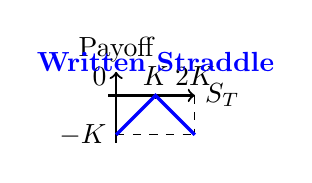
\begin{tikzpicture}[scale=1]
    % --- 定义坐标和参数 ---
    \def\K{0.5}          % 行权价 K
    \def\maxST{1}      % S_T 的最大显示范围 (稍微超过 2K)
    \def\minPayoff{-0.6} % Y轴负半轴的显示范围 (稍微超过 -K)

    % --- 绘制坐标轴 ---
    % Y 轴 (Payoff) - 主要在负半轴
    \draw[->, thick] (0, \minPayoff) -- (0, 0.3) node[above] {Payoff};
    % X 轴 (S_T)
    \draw[->, thick] (-0.1, 0) -- (\maxST, 0) node[right] {$S_T$};

    % --- 绘制辅助线和标签 ---
    % 标记原点
    \node[above left] at (0, 0) {0};

    % 在 X 轴上标记 K
    \draw (\K, 0) node[above] {$K$} -- (\K, -0.05);

    % 在 Y 轴负半轴上标记 -K (当 S_T=0 或 S_T=2K 时的收益)
    \draw (0, -\K) node[left] {$-K$} -- (0.05, -\K);

    % 绘制辅助虚线以展示对称性
    % 标记 2K 位置
    \draw (2*\K, 0) node[above] {$2K$} -- (2*\K, -0.05);
    % 从 (0, -K) 画水平虚线到 (2K, -K)
    \draw[dashed, thin] (0, -\K) -- (2*\K, -\K);
    % 从 (2K, 0) 画垂直虚线到 (2K, -K)
    \draw[dashed, thin] (2*\K, 0) -- (2*\K, -\K);


    % --- 绘制 Written Straddle 收益曲线 (蓝色粗线) ---
    % 它是 Long Straddle 的镜像，一个倒 "V" 形
    % 路径: (0, -K) -> (K, 0) -> (2K, -K) -> 延伸
    \draw[blue, very thick] (0, -\K) -- (\K, 0) -- (2*\K, -\K) -- (\maxST, \K - \maxST);

    % --- 添加描述标签 ---
    % 左侧腿的描述 (斜率为 1)
    % 右侧腿的描述 (斜率为 -1)

    % --- 添加标题标签 ---
    % 将标题放在尖峰上方
    \node[blue, anchor=south, font=\bfseries, yshift=5pt] at (\K, 0) {Written Straddle};

\end{tikzpicture}
\end{wrapfigure}